\label{sec:cinema}

Extreme scale scientific simulations are leading a charge to exascale computation, and data analytics runs the risk of being a bottleneck to scientific discovery. Due to power and I/O constraints, we expect in situ visualization and analysis will be a critical component of these workflows. 

Options for extreme scale data analysis are often presented as a stark contrast: write large files to disk for interactive, exploratory analysis, or perform in situ analysis to save detailed data about phenomena that a scientist knows about in advance. Cinema represents a novel framework for a third option – a highly interactive, data artifact-based approach that promotes exploration of simulation results, and is easily accessed through database specifications. This approach supports interactive exploration of a wide range of results, while still significantly reducing data movement and storage.

More information about the overall design of Cinema is available in the paper \textit{An Image-based Approach to Extreme Scale In Situ Visualization and Analysis} \cite{cinemaSC14}.

A Cinema Database supports the following three use cases. Taken together, these support a novel method for interactively exploring artifacts from extremely large datasets.

\begin{enumerate}
\item Searching/querying of meta-data and data artifacts. Samples can be searched purely on metadata, content, position, time, or a combination of all of these.
\item Interactive visualization of sets of data artifacts.
\item Playing interactive visualizations, allowing the user on/off control of elements in the visualization.
\end{enumerate}

\subsection{What is a Cinema Database?}
A Cinema database is a set of precomputed data artifacts that can be queried and interactively viewed. The user can decide what types of components comprise the database, based on the type of interaction that is desired with the final database.
A general design philosophy of Cinema is that applications reading and viewing a Cinema database can ignore data and determine which operations to perform. This promotes a wide range of possible interactions with the data - not just the ones imagined by the creator of the database.

Previous Cinema database specifications have concentrated on the notion that a database is a set of results sampled by visualization parameters. In this specification, we abstract this to include typical use cases from experiments by scientists. 

A scientist often has a spreadsheet with data about parameters for an experiment. This results in a set of parameters that map to a particular result - a graph, a sensor image, or other image-based data. These are a natural abstraction from previous Cinema databases. Figure \ref{fig:parametersets} shows this mapping of parameter sets to results. A collection of these mappings can be easily expressed in a Cinema database, using this specification. This is detailed in later sections.

\begin{figure}[h!]
\centering
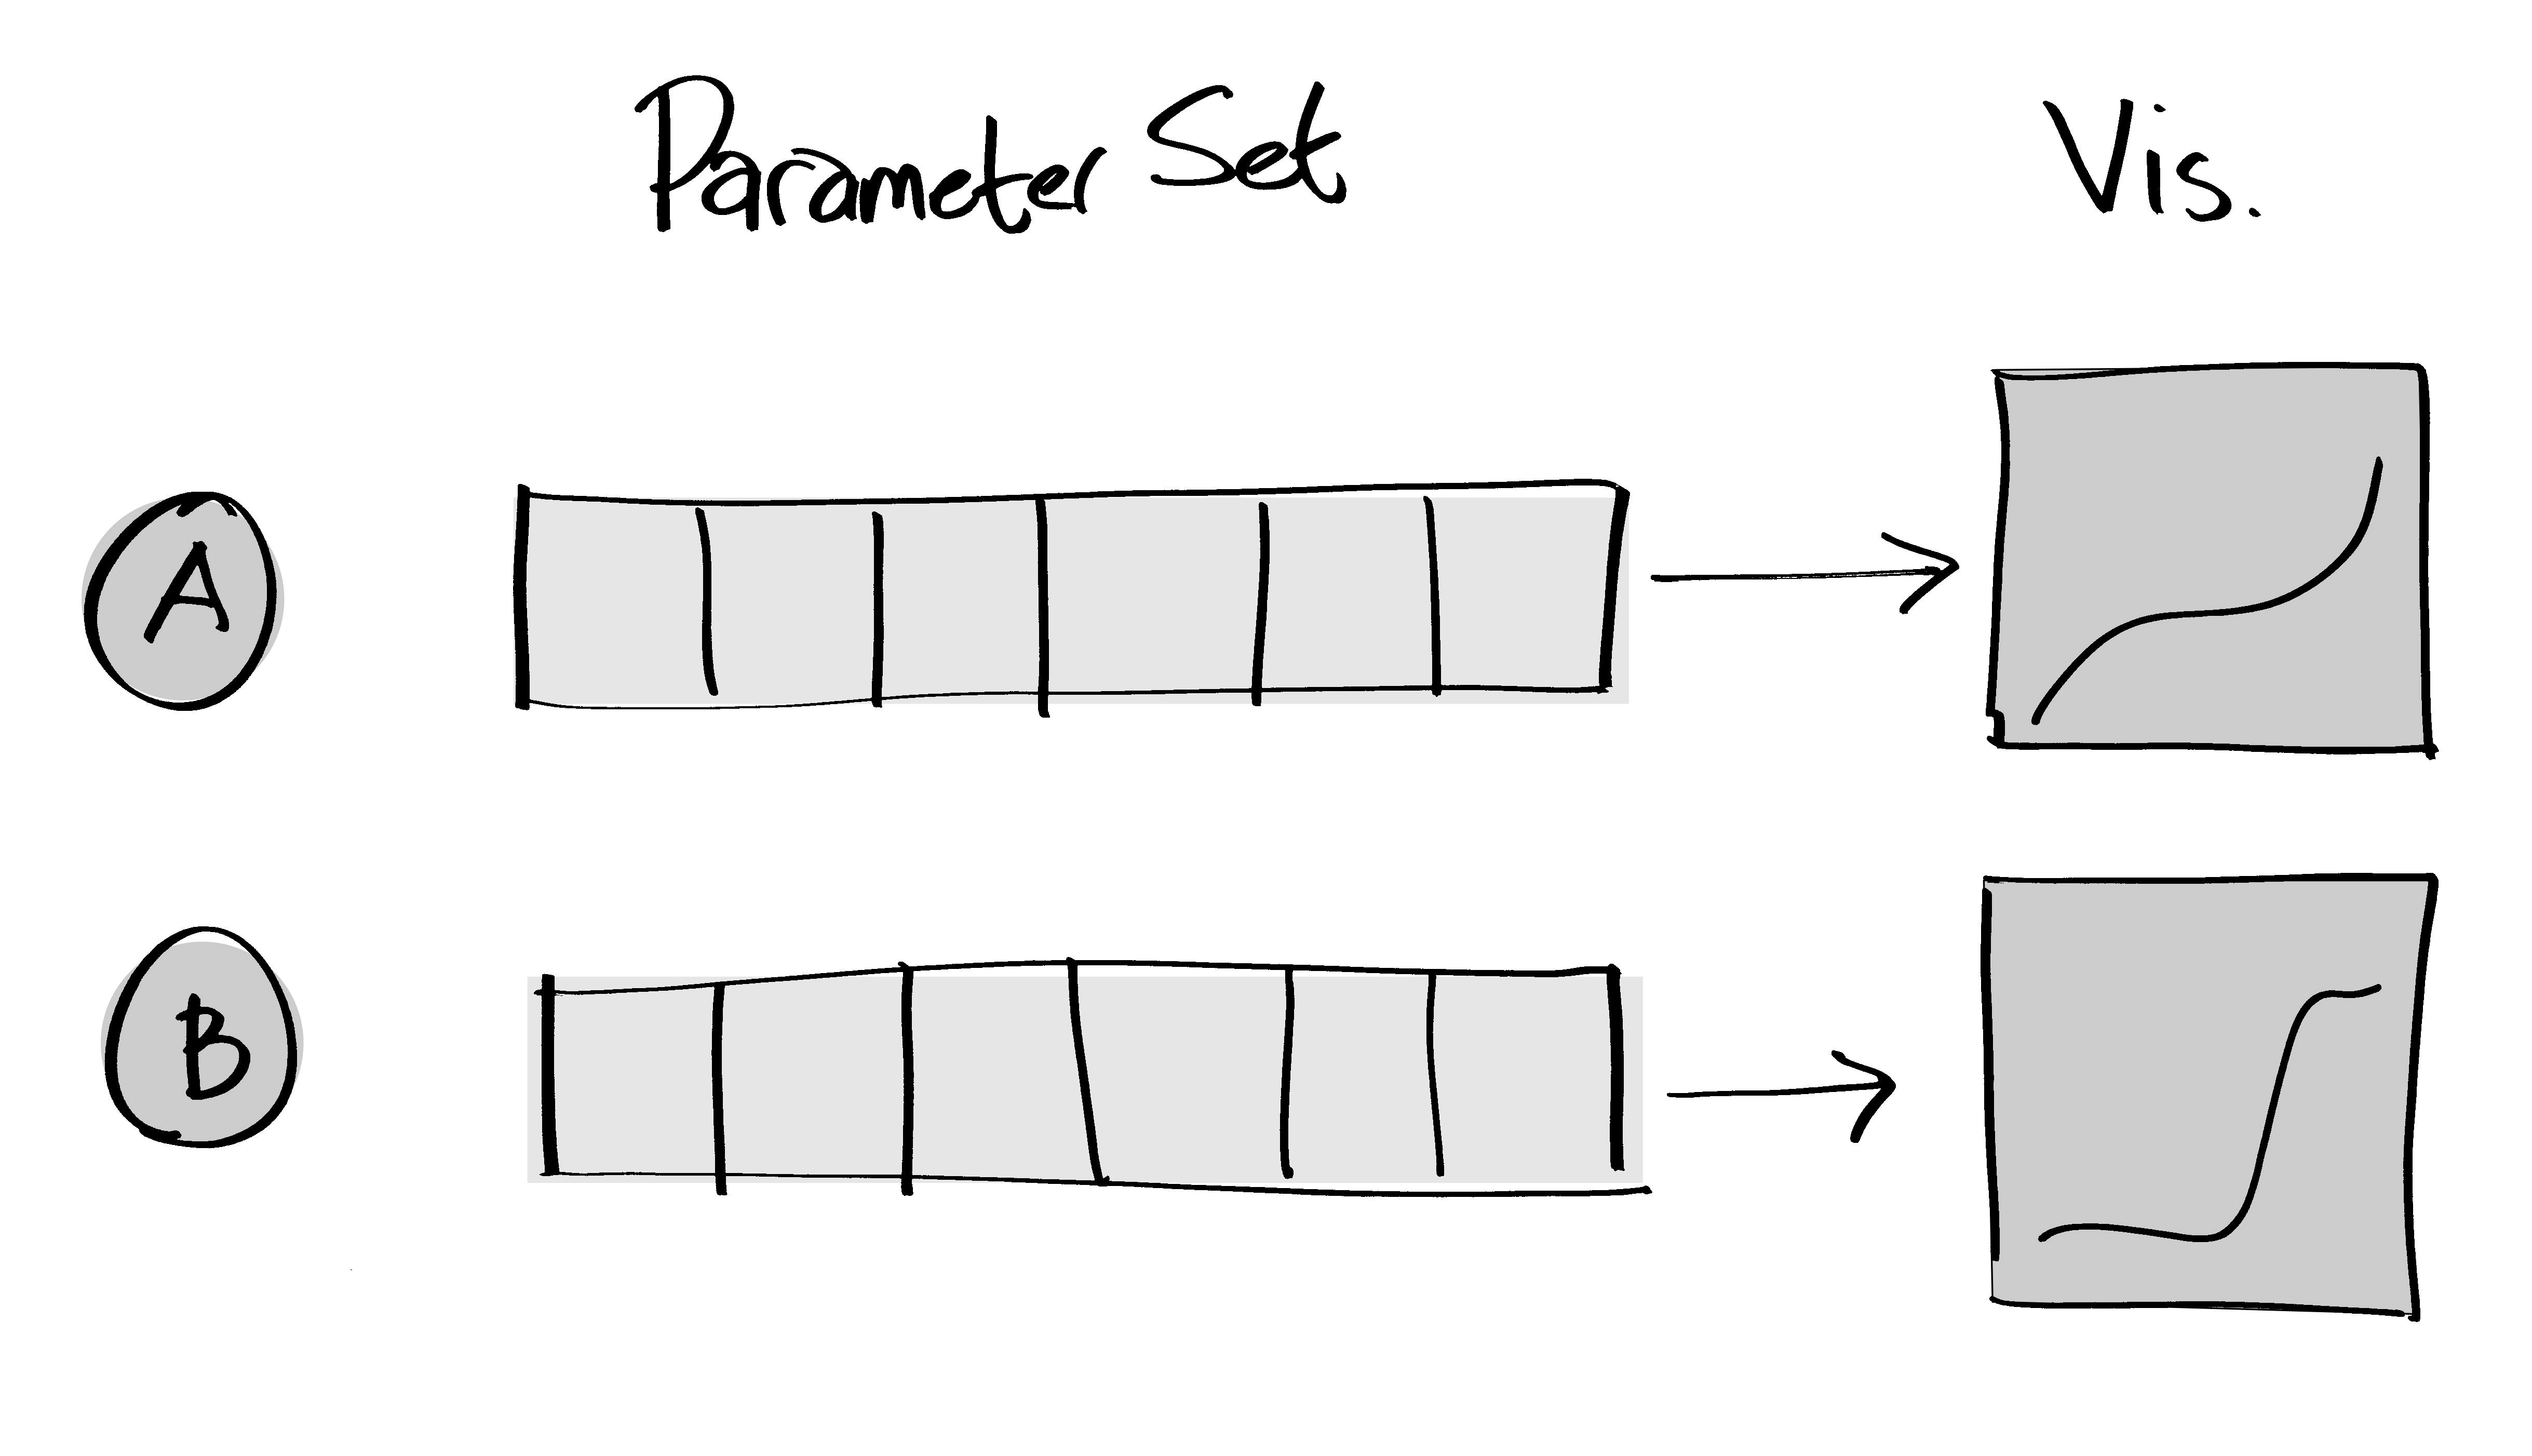
\includegraphics[width=0.8\textwidth]{img/parameter_set_diagram_filled}
\caption{
    Diagram showing a typical set of data that a scientist has for an experiment or simulations. Some set of parameters (A or B) has been used to create a visualization - a graph, an image captured from a sensor, or other data. These parameter sets can include, for example, settings on an experimental machine, inputs to a simulation, or measurements taken by a sensor. Each one of the parameter sets thus defines a unique result. Taken together, a set of these parameter sets constitutes a database of results, and a scientist often tracks this database in a spreadsheet. These parameter set/image pairings form the basis for the simplest Spec D database.
}
\label{fig:parametersets}
\end{figure}


